\subsection{Benchmark UPPAAL}\label{sub:benchmark_uppaal}
More states should intuitively mean UPPAAL runs slower, however this might not be the case if these extra states are easily pruneable.
Therefore, we tried running the same query twice in UPPAAL on a large timed word.
The timed word used in these examples is 34198 timed characters long, and the last character happens at time 238817.
The data of these benchmarks can be found on \cref{table:uppaal_benchmarks}.

\vspace{0.75em}
\begin{tabular}{|c|c|c|c|c|}
    \hline
    & States & Edges & Clocks & Time \\
    \hline
    Pruning & 6 & 8 & 3 & 76s \\
    \hline
    No pruning & 10 & 12 & 3 & 103s \\
    \hline
\end{tabular}
\captionof{table}{Table of benchmarks in UPPAAL.}
\label[table]{table:uppaal_benchmarks}
\vspace{0.75em}

As can be seen on \cref{table:uppaal_benchmarks}, checking is faster with pruning.
This points to UPPAAL not pruning the unnecessary states when checking.
So pruning not only helps with readability, it also helps with performance.

\subsection{Benchmark TREAT}\label{sub:benchmark_treat}
\subsubsection{Setup}
In the original implementation, all pruning steps were performed after generating the entire Timed Automaton (TA).
However, it might be faster if pruning is performed while generating the TA.
For this reason, we have created a series of Timed Regular Expressions (TREs) and test configurations, and put them all against each other to see how each perform.
Each configuration is a mix of pruning before and after generation of the TA.

\vspace{0.75em}
\begin{enumerate}
    \setlength\itemsep{0.5em}
    \item \textbf{N}: This configuration has no pruning.
    \item \textbf{S}: This configuration prunes only states after generation.
    \item \textbf{E}: This configuration prunes everything after generation.
    \item \textbf{SS}: This configuration prunes states during generation and only states after generation.
    \item \textbf{SE}: This configuration prunes states during generation and everything after generation.
    \item \textbf{ES}: This configuration prunes everything during generation and only states after generation.
    \item \textbf{EE}: This configuration prunes everything during generation and everything after generation.
\end{enumerate}
\vspace{0.75em}

Note: When we say prune during generation, we are talking about pruning the operands of the explosive operators.
This means the left and right operand of an intersection and the single operand of an absorbed iterator.

\vspace{.5\baselineskip plus 2pt}
As for the tests, we have generated 6 parameterized TREs, that we use to generate a total of 19 unique TREs.
Each TRE serves a unique purpose.
All these TREs can be found in \cref{app:RegularExpressionTable}.

\vspace{.5\baselineskip plus 2pt}
TREs $a$, $b$ and $f$ were all chosen because they would benefit from pruning while generating, serving as a best case scenario for SS, SE, ES and EE.
The theory is, that these configurations limit the amount of states used in the explosive operators, therefore making them less explosive.
Ideally it should make them resemble a linear complexity, since the final TAs are of constant length.

\vspace{.5\baselineskip plus 2pt}
TRE $c$, $d$ and $e$ were all chosen to benefit from no pruning while generating, serving as the best case scenario for N, S and E.
The theory is, that these TREs will not benefit from pruning while generating, since limited or no pruning can be performed during generation.

\subsubsection{Results}
The results can be split into 3 main categories.

\vspace{0.75em}
\begin{enumerate}
    \setlength\itemsep{0em}
    \item Equivalent performance between configurations.
    \item SS, SE, ES and EE configurations are better.
    \item N, S, SS configurations are better.
\end{enumerate}
\vspace{0.75em}

All the plots can be seen on \cref{sec:BenchmarkGraphs}, with all the data on \cref{sec:BenchmarkTable}, however, a few will be presented here.
On all the graphs we see the relationship between time to run/memory usage (y-axis) and a value for how long the regular expression is (x-axis). The value is explained further in \cref{sec:RegularExpressions}.

\vspace{.5\baselineskip plus 2pt}
The TREs $a$, $b$, $d$ and $e$ are all equivalent in performance.
By this we mean their graphs are all curved similarly, and they are within a few percentages of each other.
An example of this can be seen on \cref{fig:mean3-5} (this is the one with the biggest difference in this category).

\resizebox{\columnwidth}{!}{
    % 3,4,5
\plot{1,2,4}
{(1,5352.0)(2,33275.6)(4,14345441.6)}
{(1,7892.0)(2,46225.8)(4,21889111.1)}
{(1,6849.0)(2,39386.9)(4,15581794.2)}
{(1,5774.6)(2,18779.8)(4,6445558.3)}
{(1,6492.7)(2,21796.9)(4,9163154.7)}
{(1,6098.4)(2,17999.6)(4,3569375.9)}
{(1,6843.2)(2,20351.3)(4,5761799.7)}
}

\resizebox{\columnwidth}{!}{
    % 3,4,5
\plot{1,2,4}
{(1,5352.0)(2,33275.6)(4,14345441.6)}
{(1,7892.0)(2,46225.8)(4,21889111.1)}
{(1,6849.0)(2,39386.9)(4,15581794.2)}
{(1,5774.6)(2,18779.8)(4,6445558.3)}
{(1,6492.7)(2,21796.9)(4,9163154.7)}
{(1,6098.4)(2,17999.6)(4,3569375.9)}
{(1,6843.2)(2,20351.3)(4,5761799.7)}
}
\captionof{figure}{Graphs for time and memory of regular expression 3-5 ($b$).}
\label{fig:mean3-5}
\vspace{0.75em}

Since we were expecting $a$ and $b$ to be more performant on SS, SE, ES and EE, this result is not what we expected.
After inspecting one of the TAs (\cref{fig:FailedPruning}) we can see state $q1$ could have been pruned, since it can never be reached from the initial state.
However, it is not pruned, because it is neither unreachable nor dead because of the self loop.
So the pruning definitions, presented in this paper, could be more efficient by pruning patterns like this.

% File Generated Automatically
%
% NOTICE: This file has been generated automatically.
% Any manual modifications made to this file may be
% overwritten the next time it is generated.
%
% Generated by: TimedRegex, Version = 1.0.0.0
% Date 5/24/2024 10:27:37 AM
\usetikzlibrary {automata,positioning}
% "((J)+')+'"
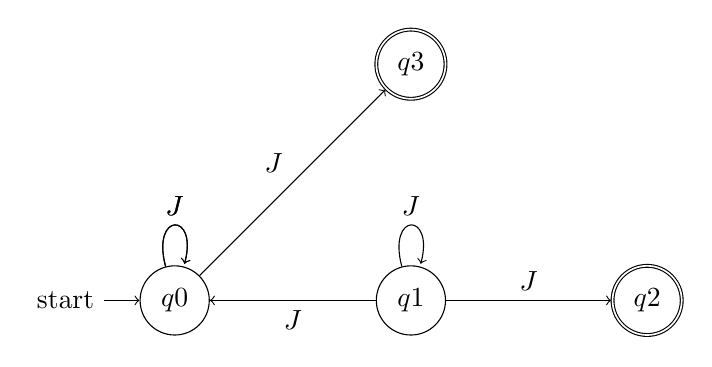
\begin{tikzpicture}[auto]
    \node[state, initial] at (6, 0)(q0){$q0$};
    \node[state] at (9, 0)(q1){$q1$};
    \node[state, accepting] at (12, 0)(q2){$q2$};
    \node[state, accepting] at (9, 3)(q3){$q3$};
    
    \path[->]
        (q1)edge node{$J$}(q2)
        (q1)edge node{$J$}(q0)
        (q0)edge node{$J$}(q3)
        (q0)edge [loop above] node{$J$}(q0)
        (q1)edge [loop above] node{$J$}(q1)
        (q0)edge [loop above] node{$J$}(q0)
        ;
\end{tikzpicture}
 

\captionof{figure}{A fully pruned TA, according to our definition, with a self loop that could be pruned.}
\label{fig:FailedPruning}
\vspace{0.75em}

Creating bigger TAs only expands on this problem. This is something that could be fixed, but that is out of the scope of this paper.

\vspace{.5\baselineskip plus 2pt}
The TRE $f$ performs better on SS, SE, ES and EE.
This graph can be seen on \cref{fig:mean15-19}.
This is the kind of performance difference we expected, and proves pruning during generation is a lot better for intersection.

\resizebox{\columnwidth}{!}{
    % 15,16,17,18,19
\plotmem{1,2,4,8,16}
{(1,2.38) (2,12.3)(4,59.38)(8,917.55)   (16,315469.2)}
{(1,4.75)(2,15.5)(4,83.24)(8,2515.32)  (16,1955655.8)}
{(1,3.73)(2,13.86)(4,62.1)(8,934.43)   (16,321366.52)}
{(1,3.73)(2,13.37)(4,33.36)(8,76.75)    (16,174.71)}
{(1,4.75)(2,14.63)(4,36.13)(8,86.02)    (16,208.98)}
{(1,3.73)(2,15.4)(4,39.59)(8,89.39)    (16,193.98)}
{(1,4.75)(2,16.66)(4,40.86)(8,90.66)    (16,195.24)}
}

\resizebox{\columnwidth}{!}{
    % 15,16,17,18,19
\plotmem{1,2,4,8,16}
{(1,2.38) (2,12.3)(4,59.38)(8,917.55)   (16,315469.2)}
{(1,4.75)(2,15.5)(4,83.24)(8,2515.32)  (16,1955655.8)}
{(1,3.73)(2,13.86)(4,62.1)(8,934.43)   (16,321366.52)}
{(1,3.73)(2,13.37)(4,33.36)(8,76.75)    (16,174.71)}
{(1,4.75)(2,14.63)(4,36.13)(8,86.02)    (16,208.98)}
{(1,3.73)(2,15.4)(4,39.59)(8,89.39)    (16,193.98)}
{(1,4.75)(2,16.66)(4,40.86)(8,90.66)    (16,195.24)}
}
\captionof{figure}{Graphs for time and memory of regular expression 15-19 ($f$).}
\label{fig:mean15-19}
\vspace{0.75em}

Finally, the TRE $c$ performs better on N, S and SS.
This graph can be seen on \cref{fig:mean6-8}
This is probably because the pruning of everything is too expensive in terms of time and memory for it to make sense for this TA.
While this is an interesting result, it does not mean these prunings are better, since they do not get rid of all the extra states, transitions and clocks.

\resizebox{\columnwidth}{!}{
    % 6,7,8
\plotmem{64,128,256}
{(64,2774.94)    (128,9617.03)     (256,36055.38)}
{(64,158752.09)  (128,1245220.51)  (256,9871874.21)}
{(64,2799.35)    (128,9667.24)     (256,36160.29)}
{(64,2338.61)    (128,8618.71)     (256,33125.43)}
{(64,14810.97)   (128,102171.73)  (256,756806.44)}
{(64,112051.15)  (128,884427.52)  (256,7031719.82)}
{(64,124523.45)  (128,977979.83)  (256,7755400.13)}
}

\resizebox{\columnwidth}{!}{
    % 6,7,8
\plotmem{64,128,256}
{(64,2774.94)    (128,9617.03)     (256,36055.38)}
{(64,158752.09)  (128,1245220.51)  (256,9871874.21)}
{(64,2799.35)    (128,9667.24)     (256,36160.29)}
{(64,2338.61)    (128,8618.71)     (256,33125.43)}
{(64,14810.97)   (128,102171.73)  (256,756806.44)}
{(64,112051.15)  (128,884427.52)  (256,7031719.82)}
{(64,124523.45)  (128,977979.83)  (256,7755400.13)}
}
\captionof{figure}{Graphs for time and memory of regular expression 6-8 ($c$).}
\label{fig:mean6-8}
\vspace{0.75em}

In conclusion, pruning by itself can lead to really explosive performance on some regular expressions, even if we prune while the automaton is generating.
However, in general, it seems like pruning during generation has the ability to turn some generations from parabolic to linear.
